\documentclass{article}

%%%%%%%%%%%%%%%%%%%%%%%%%%%%%%%%%%%%%%%%

\usepackage[utf8]{inputenc}

%%%%%%%%%%%%%%%%%%%%%%%%%%%%%%%%%%%%%%%%

\usepackage[dvipsnames]{xcolor} %may result in an error if you are using beamer with tikz. To go around it, include usenames and dvipsnames options when defining the document class, e.g. \documentclass[usenames,dvipsnames]{beamer}
\usepackage{tikz}
\usepackage{pgfplots}
\pgfplotsset{compat=1.5}

%\usetikzlibrary{external}
%\tikzexternalize
%\tikzsetexternalprefix{tikzexternal/}

%%%%%%%%%%%%%%%%%%%%%%%%%%%%%%%%%%%%%%%%

\usepackage{amsmath,amsfonts,amssymb}
\renewcommand{\baselinestretch}{1.0}
\usepackage{graphicx}
\usepackage[colorlinks=true, allcolors=blue]{hyperref}
\usepackage{color, colortbl}
\usepackage{lscape}
\usepackage{enumitem}
%\usepackage{chngcntr}
%\counterwithin{figure}{section}
%\counterwithin{table}{section}
\usepackage{booktabs,caption}
\usepackage[flushleft]{threeparttable}

%%%%%%%%%%%%%%%%%%%%%%%%%%%%%%%%%%%%%%%%

\setlength{\parindent}{0pt}
\setlength{\parskip}{\medskipamount}

%%%%%%%%%%%%%%%%%%%%%%%%%%%%%%%%%%%%%%%%

\usepackage{newtxtext,newtxmath}

% Instead of the above, use this for arXiv:

%\usepackage{txfonts}
%\usepackage{textcomp}
%\usepackage{eurosym}
%\let\texteuro\euro

%%%%%%%%%%%%%%%%%%%%%%%%%%%%%%%%%%%%%%%%

\newcommand{\unit}[1]{\ensuremath{\mathrm{#1}}}
\newcommand{\micron}{\mbox{\textmu m}}
\renewcommand{\deg}{\mbox{deg}}
\newcommand{\sqdeg}{\mbox{$\deg^2$}}
\newcommand{\persqdeg}{\mbox{$\deg^{-2}$}}
\newcommand{\arcmin}{\mbox{arcmin}}
\newcommand{\sqarcmin}{\mbox{\arcmin$^2$}}
\newcommand{\persqarcmin}{\mbox{\arcmin$^{-2}$}}
\newcommand{\arcsec}{\mbox{arcsec}}
\newcommand{\sqarcsec}{\mbox{\arcsec$^2$}}
\newcommand{\persqarcsec}{\mbox{\arcsec$^{-2}$}}
\newcommand{\sqmm}{\mbox{mm$^2$}}
\newcommand{\deighty}{\ensuremath{d_{80}}}
\newcommand{\Hs}{\mbox{$H_\mathrm{s}$}}
\newcommand{\Ravg}{\mbox{$R_\mathrm{avg}$}}
\newcommand{\Tavg}{\mbox{$T_\mathrm{avg}$}}
\newcommand{\mm}{\mbox{mm}}

\newcommand{\code}[1]{{\ttfamily #1}}

%%%%%%%%%%%%%%%%%%%%%%%%%%%%%%%%%%%%%%%%

\begin{document}

\pagestyle{empty}

\begin{center}

{\Large \bfseries DDRAGUITO: Analysis of Commissioning Data}

\vspace{2cm}

\begin{tabular}{ll}
Prepared by:&Alan M. Watson\\
Reviewed by:&\\
Approved by:&\\
%DDRAGO Reference:&Document 2\\
COLIBRÍ Reference:&COLIBRI-UNAM-???\\
Version:&1.1\\
Date:&19 July 2023\\
\end{tabular}

\vspace{\fill}

COLIBRÍ Project\\
Instituto de Astronom{\'\i}a\\
Universidad Nacional Aut\'onoma de M\'exico

\end{center}

\clearpage

\clearpage
\section*{Version History}

\begin{itemize}

\item Version 1.1 of 19 July 2023

\begin{itemize}
\item Reworked since we realized that the filters were installed in the order $grizy$ but configured in TCS in the order $rgizy$. Thus, all of the images we thought were in $g$ were actually in $r$ and vice versa.
\item Automated the photometry for the zero-points.
\end{itemize}

\item Version 1.0 of 12 July 2023

\begin{itemize}
    \item Initial version.
\end{itemize}

\end{itemize}

%%%%%%%%%%%%%%%%%%%%%%%%%%%%%%%%%%%%%%%%%

\clearpage
%%%%%%%%%%%%%%%%%%%%%%%%%%%%%%%%%%%%%%%%%

\pagestyle{plain}

\setcounter{tocdepth}{2}
\tableofcontents
\clearpage

%\listoffigures
%\clearpage

%\listoftables
%\clearpage

%%%%%%%%%%%%%%%%%%%%%%%%%%%%%%%%%%%%%%%%%

\section{Introduction}

The DDRAGUITO instrument was commissioned on the COLIBRI telescope at OHP in 2023 March and April. The work was carried out by François Dolon, Damien Dornic, Johan Floriot, and Simona Lombardo working on-site and Alan Watson working remotely.

This document concentrates on the performance of the instrument on the telescope. A companion document \cite{laboratory} describes the detector and filter wheel verification in the laboratory. A second companion document \cite{dolon} describes in detail the engineering work performed, in particular the verification of the instrument upon unpacking, the balancing and installation, the pumping-down, and the recharging of the refrigerant.

\section{Filters}

During commissioning, the $g$, $r$, $i$, $z$, and $y$ filters were installed. The $gri$, $zy$, and $B$ were not installed.

Unfortunately, there was some confusion about the order in which there were installed. Prior to commissioning, we believed they were installed in slots 0-4 in the order $rgizy$. TCS was configured with this understanding, all of the tests were run with this understanding, and all of the contemporaneous notes on the commissioning run were written with this understanding.

However, subsequently we have come to believe that the filters were installed in the order $grizy$. The evidence for this is:

\begin{enumerate}
    \item A photograph showing the filters in slots 0 and 1 in reflected light. We know the light is reflected, since we can see an image of the camera. The filter in slot 0 has an orange color and the filter in slot 1 has a blue color. The $g$ filter reflects above 550~nm and so is expected to be orange. The $r$ filter reflects below 550~nm and so is expected to be blue. (Note that the colors in transmitted light would be reversed.)
    \item If we assume the order is $grizy$, then the color terms in the transformation from instrumental to standard magnitudes are are relatively small, being about $-0.1(g-r)$ in $g$ and about $+0.01(g-r)$ in $r$. If we assume the order is $rgizy$, the color terms are $+0.85(g-r)$ and $-0.96(g-r)$. These color terms are telling us that the filter in slot 0 is more similar to $g$ than to $r$ an the filter in slot 1 is more similar to $r$ than to $g$.
    \item If we assume the order in $grizy$, then the ratio of measured to expected zero points drops smoothly from $i$ to $r$ to $g$. If we assume the order is $rgizy$, the efficiency drops by a factor of two from $i$ to $r$ but then increases by a factor of two from $r$ to $g$. It is easy to understand the efficiency decreasing to the blue because of old coatings on the mirrors. It is very difficult to explain why the efficiency in $g$ should be significantly higher than the efficiency in $r$.
    \item In one band only, the flat fields show diagonal stripes possible from the substrate. We we assume the order is $grizy$, these stripes are in $g$. Our experience is that features in the substrate often appear in the blue. Since $g$ is the bluest filter, it is reasonable that the stripes appear in it but not in any of the redder filters. If we assume the order is $rgizy$, these stripes are in $r$, but not in the blue filter $g$ or the redder filter $i$, which is difficult to explain.
\end{enumerate}

In the analysis we present here, we will assume that the filter order is $grizy$. However, we have not altered the contemporaneous notes reproduced in Appendix~\ref{appendix:notes}.

TCS records the filter in the header of the FITS images. We believe that where the header states that the filter was $g$, it was actually $r$, and that where the header states that the filter was $r$, it was actually $g$.

\clearpage
\section{Dates}

TCS works internally in UTC. At the time of commissioning, the civil time CET was one hour ahead of UTC. For convenience, the correspondence between UTC and MJD during the commissioning run is given in Table~\ref{table:dates}.

\begin{table}[pb]
\caption{Dates}
\label{table:dates}
\begin{center}
\begin{tabular}{lll}
\hline
UTC&MJD\\
\hline
2023-03-10 00:00:00&60013.0\\
2023-03-11 00:00:00&60014.0\\
2023-03-12 00:00:00&60015.0\\
2023-03-13 00:00:00&60016.0\\
2023-03-14 00:00:00&60017.0\\
2023-03-15 00:00:00&60018.0\\
2023-03-16 00:00:00&60019.0\\
2023-03-17 00:00:00&60020.0\\
2023-03-18 00:00:00&60021.0\\
2023-03-19 00:00:00&60022.0\\
2023-03-20 00:00:00&60023.0\\
2023-03-21 00:00:00&60024.0\\
2023-03-22 00:00:00&60025.0\\
2023-03-23 00:00:00&60026.0\\
2023-03-24 00:00:00&60027.0\\
2023-03-25 00:00:00&60028.0\\
2023-03-26 00:00:00&60029.0\\
2023-03-27 00:00:00&60030.0\\
2023-03-28 00:00:00&60031.0\\
2023-03-29 00:00:00&60032.0\\
2023-03-30 00:00:00&60033.0\\
2023-03-31 00:00:00&60034.0\\
2023-04-01 00:00:00&60035.0\\
2023-04-02 00:00:00&60036.0\\
2023-04-03 00:00:00&60037.0\\
2023-04-04 00:00:00&60038.0\\
2023-04-05 00:00:00&60039.0\\
2023-04-06 00:00:00&60040.0\\
2023-04-07 00:00:00&60041.0\\
2023-04-08 00:00:00&60042.0\\
2023-04-09 00:00:00&60043.0\\
2023-04-10 00:00:00&60044.0\\
2023-04-11 00:00:00&60045.0\\
2023-04-12 00:00:00&60046.0\\
2023-04-13 00:00:00&60047.0\\
2023-04-14 00:00:00&60048.0\\
2023-04-15 00:00:00&60049.0\\
\hline
\end{tabular}
\end{center}
\end{table}

\clearpage
\section{Cryogenic Performance}

The cryogenic system uses PT-30 gas a refrigerant.
The compressor has lost significant PT-30 pressure during June 2022, but was recharged from a tank prior to the commissioning run \cite[p.~17]{dolon}. The recharge raised the pressure from 110~PSI to 220~PSI. However, when the tank was disconnected there was a leak and the pressure dropped to 178 PSI. This is significantly below the nominal pressure is 280~PSI \cite[p.~4]{service-cabinet}.

Nevertheless, we started cooling at 2023-03-14 15:40 UTC (MJD 60017.6528). Figure~\ref{figure:cool-down} shows that the detector and cold-head reacher their set-point temperatures of $-110$~C and $-130$~C in under three hours.

\begin{figure}[pb]
\begin{center}
\includegraphics[width=0.7\columnwidth]{figures/cool-down.pdf}
\medskip
\caption{The detector and cold-end temperatures during the cool-down.}
\label{figure:cool-down}
\end{center}
\end{figure}

\begin{figure}[pb]
\begin{center}
\includegraphics[width=0.7\columnwidth]{figures/warm-up.pdf}
\medskip
\caption{The detector and cold-end temperatures during the warm-up.}
\label{figure:warm-up}
\end{center}
\end{figure}

We then cooled continuously until 2023-04-11 11:28 UTC (MJD 60045.4778). Figure~\ref{figure:warm-up} shows that the detector and cold-head warmed-up in about two hours.

\begin{figure}[pb]
\begin{center}
\includegraphics[width=0.7\columnwidth]{figures/temperature-stability-a.pdf}
\medskip
\caption{The detector temperatures during commissioning. Note the occasional episodes during which the detector warms to up to $-90$~C.}
\label{figure:temperature-stability-a}
\end{center}
\end{figure}

\begin{figure}[pb]
\begin{center}
\includegraphics[width=0.7\columnwidth]{figures/temperature-stability-b.pdf}
\medskip
\caption{The detector temperatures during commissioning. Outside of the warming episodes, the detector is stable to $\pm0.1$~C.}
\label{figure:temperature-stability-b}
\end{center}
\end{figure}

Figure~\ref{figure:temperature-stability-a} and \ref{figure:temperature-stability-b} show that the detector temperature was typically stable to $\pm0.1$~C (the resolution of the temperature sensor) except for a few episodes when the detector warmed-up significantly, to $-90$~C in one case. The cold-end temperature rose too during these episodes, which suggests a lack of cooling power.

\begin{figure}[pb]
\begin{center}
\includegraphics[width=0.7\columnwidth]{figures/refrigerant-pressure.pdf}
\medskip
\caption{The refrigerant pressure during commissioning.}
\label{figure:refrigerant-pressure}
\end{center}
\end{figure}

Figure~\ref{figure:refrigerant-pressure} shows that the refrigerant pressure does not show corresponding anomalies during these episodes. As expected, the supply pressure (190--240 PSI) is greater than the equalized pressure and the return pressure (15--25 PSI) is lower. Both pressures show diurnal trends, presumably related to temperature changes.

\begin{figure}[pb]
\begin{center}
\includegraphics[width=0.7\columnwidth]{figures/temperature-stability-c.pdf}
\medskip
\caption{The detector and weather station temperatures during commissioning. The detector temperature is shifted by 110 C. Note that the warming episodes occur at night when the temperature drops. (There is no weather data after 2023-04-06 08:13 UTC because of an apparent failure in the script that queries the PLC.)}
\label{figure:temperature-stability-c}
\end{center}
\end{figure}

However, Figure~\ref{figure:temperature-stability-c} shows that the warming episodes occur during the night and the worst episode occurs on the coldest night when the weather station measured temperatures around 0~C. The correspondence is not perfect -- the first episodes occur on relatively warm nights with temperatures of around 8~C -- but is very suggestive. 

The manual for the service cabinet gives the operating temperature range as 20--30~C \cite[p.~7]{service-cabinet}, and if the temperatures in the tent are similar to those measured by the weather station, then we were likely operating the service cabinet outside of its specified operating range during much of the commissioning run.

Our working hypothesis is that these warming episodes were caused by operating the service cabinet at low ambient temperatures. At OAN, the service cabinet will be in a temperature-controlled environment and we suggest that we are unlikely to encounter this problem. It might also be that the system is better behaved when the refrigerant pressure is higher.

In subsequent analysis, we will only consider images taken when the detector temperature at the start and end of the exposure (\verb|SDTTM| and \verb|EDTTM| in the header) are $-110\pm0.1$~C.

\clearpage
\section{Chamber Pressure}

On 2023 March 13 the detector chamber was pumped-down from 0.3~mbar to $9.33\times10^{-3}$~mbar.
Figure~\ref{figure:chamber-pressure} shows that the chamber pressure was stable at about $3\times10^{-3}$~mbar while the detector was cold.

However, when the detector warmed-up it rose to a peak pressure of about 1~mbar and a steady pressure of about 0.2~mbar. This is much larger than the pressure prior to cooling.

The camera firmware will not operate the compressor if the chamber pressure is above 0.5~Torr (0.67~mbar). Thus, despite losing vacuum to a large degree, it should have been possible to cool the camera again.

\begin{figure}[pb]
\begin{center}
\includegraphics[width=0.7\columnwidth]{figures/chamber-pressure.pdf}
\medskip
\caption{The chamber pressure during commissioning.}
\label{figure:chamber-pressure}
\end{center}
\end{figure}

\clearpage
\section{Detector Format}

\begin{figure}[p]
\begin{center}
\begin{tikzpicture}[scale=24]
\draw (-0.2098,-0.2056) -- (+0.2098,-0.2056) -- (+0.2098,+0.2056) -- (-0.2098,+0.2056) -- cycle;
\draw (-0.2048,-0.2056) -- (+0.2048,-0.2056) -- (+0.2048,+0.2056) -- (-0.2048,+0.2056) -- cycle;
\draw [dotted] (-0.2098,0) -- (+0.2098,0);
\draw [dotted] (0,-0.2056) -- (0,+0.2056);
\draw[->] (-0.025,-0.025) -- (-0.025,-0.175) -- (-0.175,-0.175);
\draw[->] (+0.025,-0.025) -- (+0.025,-0.175) -- (+0.175,-0.175);
\draw[->] (-0.025,+0.025) -- (-0.025,+0.175) -- (-0.175,+0.175);
\draw[->] (+0.025,+0.025) -- (+0.025,+0.175) -- (+0.175,+0.175);
\draw (-0.12,-0.12) node {0};
\draw (+0.12,-0.12) node {1};
\draw (-0.12,+0.12) node {2};
\draw (+0.12,+0.12) node {3};
\draw[->] (-0.2,-0.25) -- (+0.2,-0.25) node [anchor=west] {$x$};
\draw[->] (-0.25,-0.2) -- (-0.25,+0.2) node [anchor=south] {$y$};
\draw[dashed] (-0.2096,-0.2048) -- (-0.2096,+0.2048) -- (+0.2096,+0.2048) -- (+0.2096,-0.2048) -- cycle; 
\draw[dashed] (-0.1024,-0.1024) -- (-0.1024,+0.1024) -- (+0.1024,+0.1024) -- (+0.1024,-0.1024) -- cycle; 
\draw[dashed] (-0.0512,-0.0512) -- (-0.0512,+0.0512) -- (+0.0512,+0.0512) -- (+0.0512,-0.0512) -- cycle; 
\end{tikzpicture}
\caption{The format of the CCD. The full format is an active area is $4096~\mbox{columns} \times 4112~\mbox{rows}$ and with 50 columns of underscan at the start and end of each row, giving a total format of $4196~\mbox{columns} \times 4112~\mbox{rows}$. It is read in four quadrants, as shown by the dotted line and the arrows. The parallel clocks move charge vertically and the serial clocks move charge horizontally. The quadrants are numbered 0 to 3 as shown. The dashed lines show the \code{4kx4k}, \code{2kx2k}, and \code{1kx1k} windows.}
\label{figure:format}
\end{center}
\end{figure}

The detector has a active area of  $4096~\mbox{columns} \times 4112~\mbox{rows}$. It is read using the “split full frame read-out through four amplifiers” scheme \cite[p.~17]{e2v} with 50 columns of underscan at the start and end of each row, giving a total size of $4196~\mbox{columns} \times 4112~\mbox{rows}$. This is show in Figure~\ref{figure:format}

The SI Image software allows us to define windows provided they are centered on the detector. We define three windows that we expect will be useful for science, named \code{4kx4k}, \code{2kx2k}, and \code{1kx1k}, described below and shown in Figure~\ref{figure:format}. Each window can be used with a binning of 1, 2, or 4 pixels (both vertically and horizontally).

The \code{4kx4k} window has an active area of $4096~\mbox{columns} \times 4096~\mbox{rows}$, centered on the detector, with 48 columns of underscan at the start and end of each row, giving a total size of $4192~\mbox{columns} \times 4096~\mbox{rows}$.

The \code{2kx2k} window has an active area of $2048~\mbox{columns} \times 2048~\mbox{rows}$, centered on the detector, without underscan.

The \code{1kx1k} window has an active area of $1024~\mbox{columns} \times 1024~\mbox{rows}$, centered on the detector, without underscan.

We do not typically use the full native format. In the laboratory, the first and last rows showed unusual behavior (higher values in the underscan regions and lower values in the active regions) \cite{laboratory}. Also, the underscans of 50 columns are not commensurate with a binning of 4.  However, the full native format is available as an engineering mode with window name \verb|full|.

\clearpage
\section{Detector Read Modes}

The controller offers three read frequencies (1.01~MHz, 502.5~kHz, and 332.2~kHz) and two gain modes (low and high). These are exposed by TCS as “read modes” and are summarized in Table~\ref{table:read-modes}. 

We expect the most useful read mode for our applications will be read mode 0, which combines fast readout (7 seconds), reasonable read noise (6--7 electrons), and the deepest full-well (about 140,000 electrons) \cite{laboratory}. All data taken during commissioning were taken with this read mode.

\begin{table}[pb]
\begin{center}
\caption{Read Modes}
\label{table:read-modes}
\medskip    
\begin{tabular}{ccc}
\hline
Read Mode&Frequency&Gain\\
\hline
\code{0}&1.01~MHz&low\\
\code{1}&1.01~MHz&high\\
\code{2}&502.5~kHz&low\\
\code{3}&502.5~kHz&high\\
\code{4}&332.2~kHz&low\\
\code{5}&332.2~kHz&high\\
\hline
\end{tabular}
\end{center}
\end{table}

\clearpage
\section{Underscan Level}

During commissioning we took many sequences of 10 biases. For those biases with binning 1 taken at night and with a detector temperature of $-110\pm0.1$~C, we calculated the mean level in the underscan region of each quadrant with $3\sigma$ rejection (i.e., using \verb|astropy.stats.sigma_clip_stats|).

\begin{figure}[pb]
\begin{center}
\includegraphics[width=0.7\columnwidth]{figures/underscan-time.pdf}
\medskip
\caption{The underscan values over the commissioning run.}
\label{figure:underscan-time}
\end{center}
\end{figure}

\begin{figure}[pb]
\begin{center}
\includegraphics[width=0.7\columnwidth]{figures/underscan-relative-0.pdf}
\medskip
\caption{The underscan values relative to quadrant 0 over the commissioning run.}
\label{figure:underscan-relative-0}
\end{center}
\begin{center}
\includegraphics[width=0.7\columnwidth]{figures/underscan-relative-1.pdf}
\medskip
\caption{The underscan values relative to quadrant 1 over the commissioning run.}
\label{figure:underscan-relative-1}
\end{center}
\end{figure}

Figure~\ref{figure:underscan-time} shows the variation of the underscan values over the whole commissioning run. There is clear variation in the value at the level of a few DN both during and between nights. Figures~\ref{figure:underscan-relative-0} and \ref{figure:underscan-relative-1} show the relative values of the underscan with respect to quadrants 0 and 1, and show that to a large degree quadrants 2 follows quadrant 0 and and quadrant 3 follows quadrant 1. That is, the left and right quadrants vary together. 

\begin{figure}[pb]
\begin{center}
\includegraphics[width=0.7\columnwidth]{figures/underscan-temperature.pdf}
\medskip
\caption{The underscan values against the weather temperature over the commissioning run.}
\label{figure:underscan-temperature}
\end{center}
\end{figure}

\begin{figure}[pb]
\begin{center}
\includegraphics[width=0.7\columnwidth]{figures/underscan-residual-temperature.pdf}
\medskip
\caption{The residuals of the underscan values after removing a quadratic model in temperature.}
\label{figure:underscan-residual-temperature}
\end{center}
\begin{center}
\includegraphics[width=0.7\columnwidth]{figures/underscan-residual-time.pdf}
\medskip
\caption{The residuals of the underscan values after removing a quadratic model in temperature.}
\label{figure:underscan-residual-time}
\end{center}
\end{figure}

Figure~\ref{figure:underscan-temperature} shows that a large component of this variation is due to temperature. We fit each the values in each quadrant with a quadratic and show the residuals against temperature and time in Figures~\ref{figure:underscan-residual-temperature} and \ref{figure:underscan-residual-time}. It's clear that this model removes the general trend with temperature, but the residuals shows that clearly there are other currently unidentified factors at play. The largest residuals are on the first night  and then at the start of some subsequent nights.

This variation of the underscan values confirm that the reduction pipeline should calculate and subtract them from each image individually. This is not unexpected.

\clearpage
\section{Residual Bias}

As mentioned in the previous section, during commissioning we took many sequences of 10 biases. For those biases in the 280 sequences with binning 1 taken at night and with a detector temperature of $-110\pm0.1$~C, we calculated the mean level in the underscan region of each quadrant with $3\sigma$ rejection, subtracted these values from the corresponding quadrants, and determined the residual bias level in each quadrant again using the mean with $3\sigma$ rejection.

\begin{figure}[pb]
\begin{center}
\includegraphics[width=0.7\columnwidth]{figures/bias-residual-sequence.pdf}
\medskip
\caption{The mean values of the residual in each quadrant as a function of the index in the sequence of 10 biases. The error bars indicate the standard deviation of the values about the mean.}
\label{figure:bias-residual-sequence}
\end{center}
\end{figure}

\begin{figure}[pb]
\begin{center}
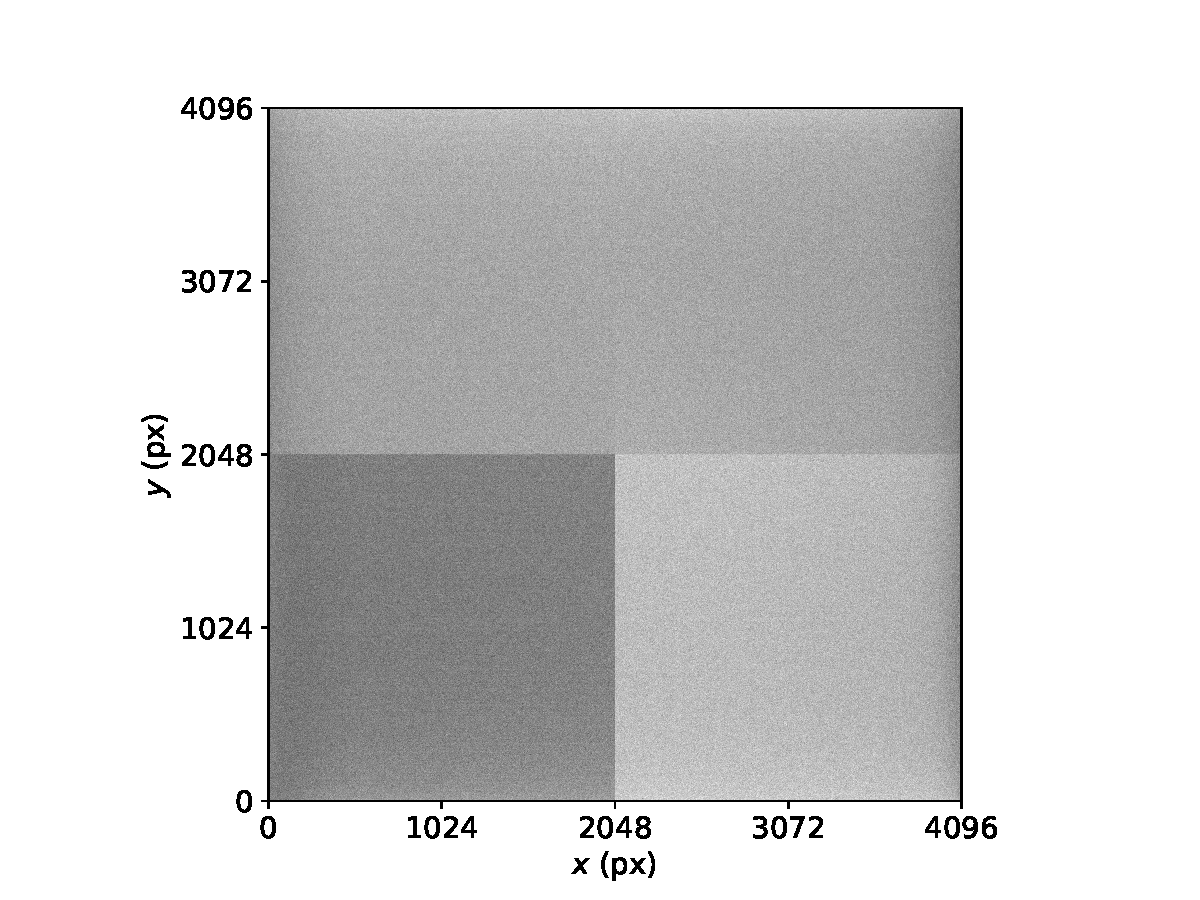
\includegraphics[width=0.7\columnwidth]{figures/bias-a.pdf}
\medskip
\caption{Residual bias image formed the first images in 280 sequences of 10 bias images. The gray scale is $(-1,+1)$ DN.}
\label{figure:bias-a}
\end{center}
\begin{center}
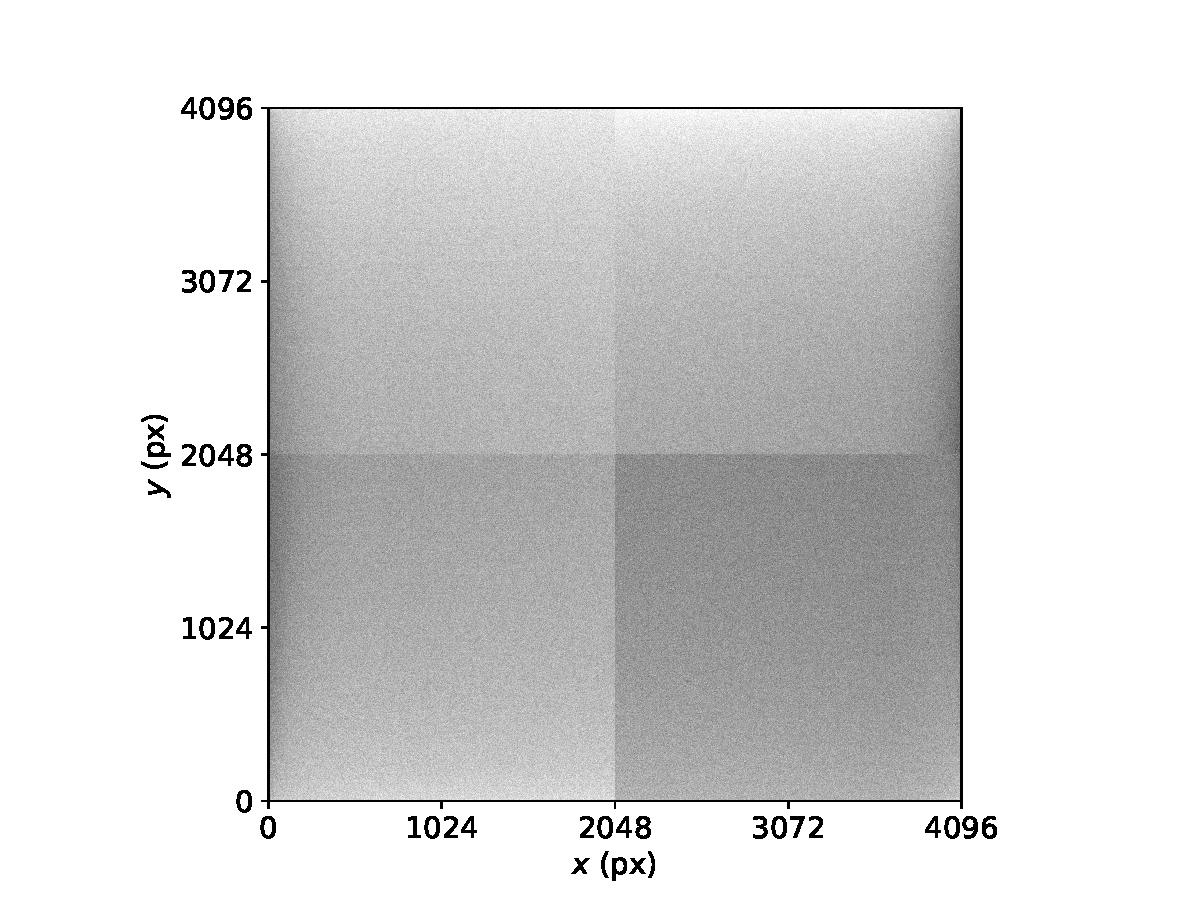
\includegraphics[width=0.7\columnwidth]{figures/bias-b.pdf}
\medskip
\caption{Residual bias image formed the last images in 280 sequences of 10 bias images. The gray scale is $(-1,+1)$ DN.}
\label{figure:bias-b}
\end{center}
\end{figure}

\begin{figure}[pb]
\begin{center}
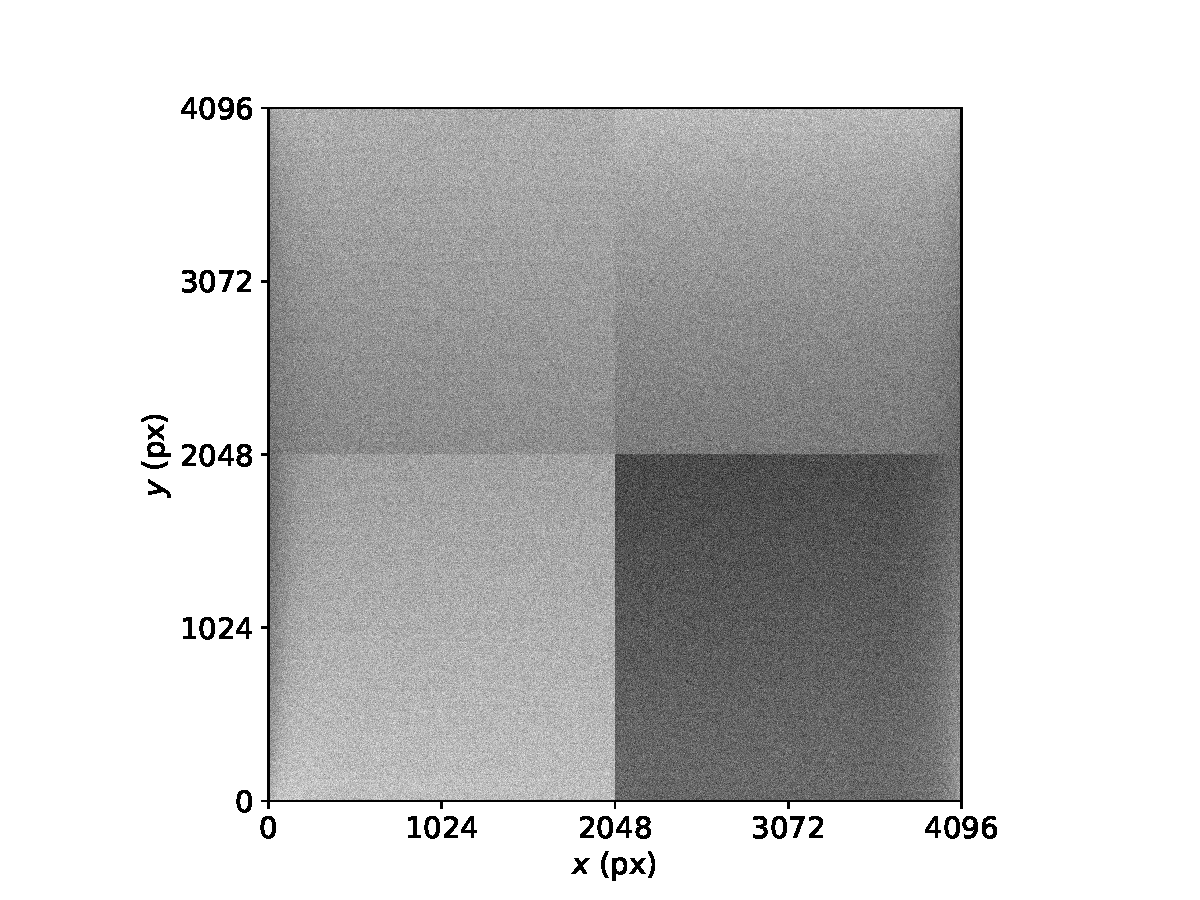
\includegraphics[width=0.7\columnwidth]{figures/bias-diff.pdf}
\medskip
\caption{Difference between the residual bias images formed the last and first images in 280 sequences of 10 bias images. The gray scale is $(-1,+1)$ DN.}
\label{figure:bias-diff}
\end{center}
\end{figure}

\begin{figure}[pb]
\begin{center}
\includegraphics[width=0.7\columnwidth]{figures/bias-diff-y.pdf}
\medskip
\caption{The mean values in the $x$ direction of the difference between the residual bias images formed the last and first images in 280 sequences of 10 bias images.}
\label{figure:bias-diff-y}
\end{center}
\begin{center}
\includegraphics[width=0.7\columnwidth]{figures/bias-diff-x.pdf}
\medskip
\caption{The mean values in the $y$ direction of the difference between the residual bias images formed the last and first images in 280 sequences of 10 bias images.}
\label{figure:bias-diff-x}
\end{center}
\end{figure}

We found that the residual bias level changed in a systematic way during the sequences of 10 biases. Figure~\ref{figure:bias-residual-sequence} shows the mean values of the residual in each quadrant as a function of the index in the sequence of 10 biases. The error bars indicate the standard deviation of the values about the mean and the errors in the mean are a factor of $\sqrt{280} \approx 17$ smaller, so these changes are very significant. 

Figures~\ref{figure:bias-a} and \ref{figure:bias-b} show residual bias images formed from the first and last images in sequences of 10 bias images. Figure~\ref{figure:bias-diff} shows the difference. Figures~\ref{figure:bias-diff-y} and \ref{figure:bias-diff-x} show the means in the difference images in the $x$ and $y$ directions. We see that despite being significant, these residuals are small. The largest are about $\pm0.5$~DN, which corresponds to $\pm1$ electron. Nevertheless, they have structure and are not simply changes in the pedestal value.

\begin{figure}[pb]
\begin{center}
\includegraphics[width=0.7\columnwidth]{figures/dark-60-residual-sequence.pdf}
\medskip
\caption{The mean values of the residual in each quadrant as a function of the index in the sequence of 5 darks with exposure times of 60 seconds. The error bars indicate the standard deviation of the values about the mean.}
\label{figure:dark-60-residual-sequence}
\end{center}
\end{figure}

\begin{figure}[pb]
\begin{center}
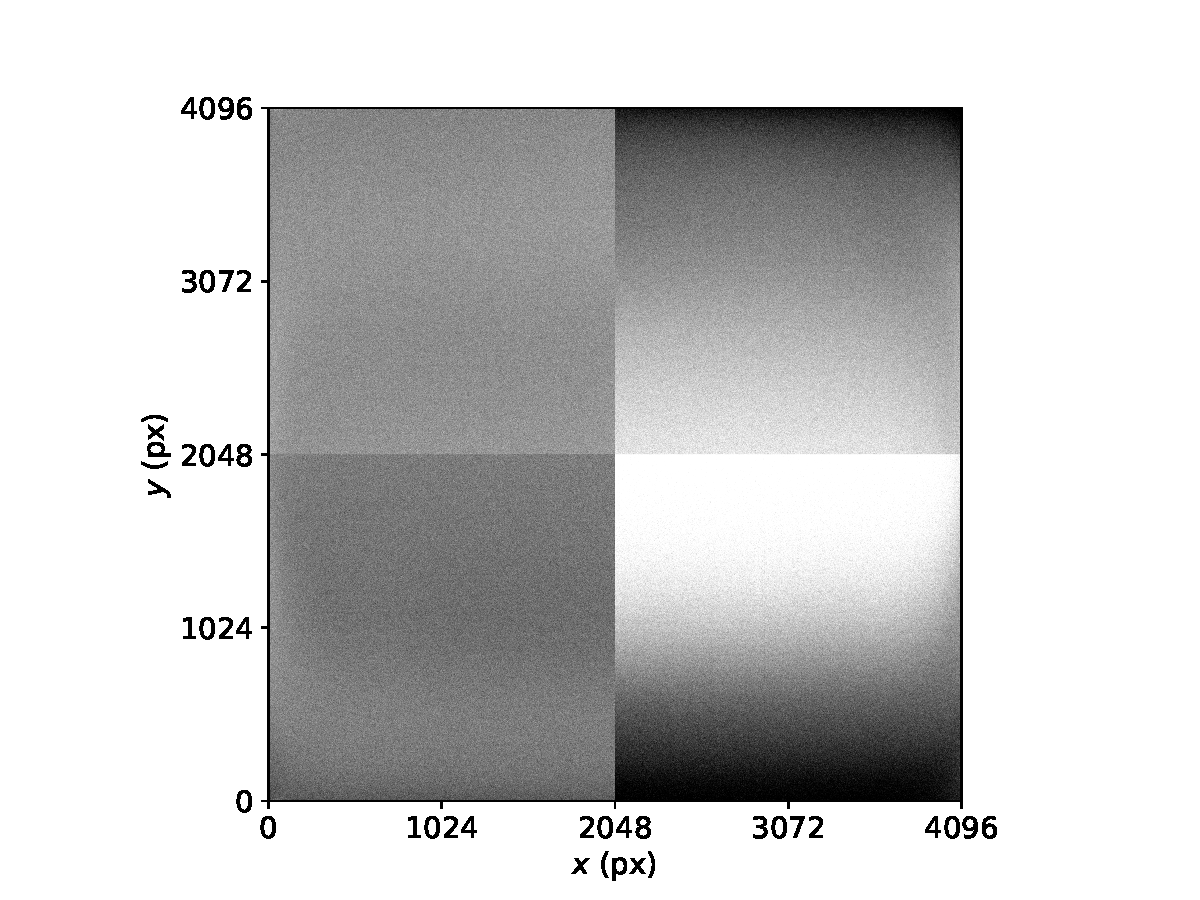
\includegraphics[width=0.7\columnwidth]{figures/dark-60-a.pdf}
\medskip
\caption{Residual bias image formed the first images in 280 sequences of 5 dark images with exposure times of 60 seconds. The gray scale is $(-1,+1)$ DN.}
\label{figure:dark-60-a}
\end{center}
\begin{center}
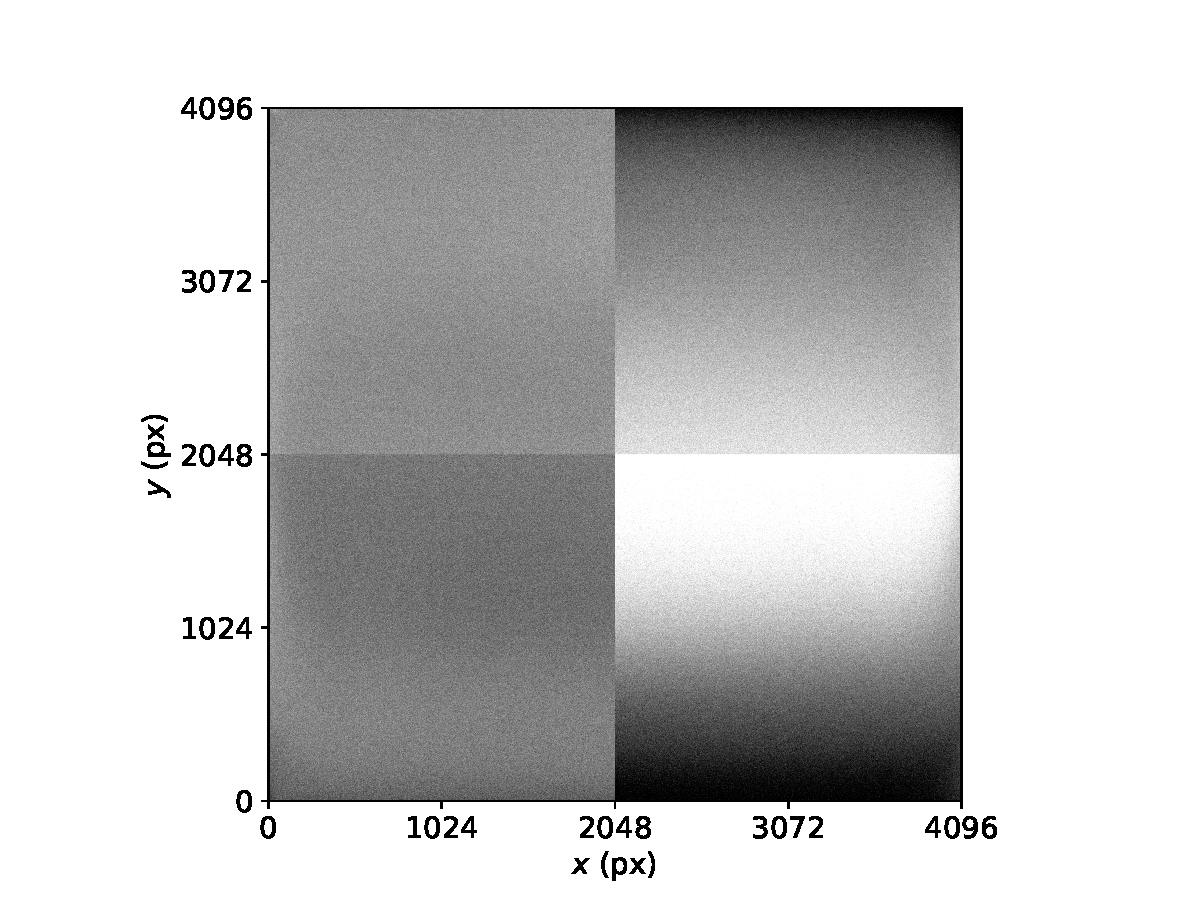
\includegraphics[width=0.7\columnwidth]{figures/dark-60-b.pdf}
\medskip
\caption{Residual bias image formed the last images in 280 sequences of 5 dark images with exposure times of 60 seconds. The gray scale is $(-1,+1)$ DN.}
\label{figure:dark-60-b}
\end{center}
\end{figure}

\begin{figure}[pb]
\begin{center}
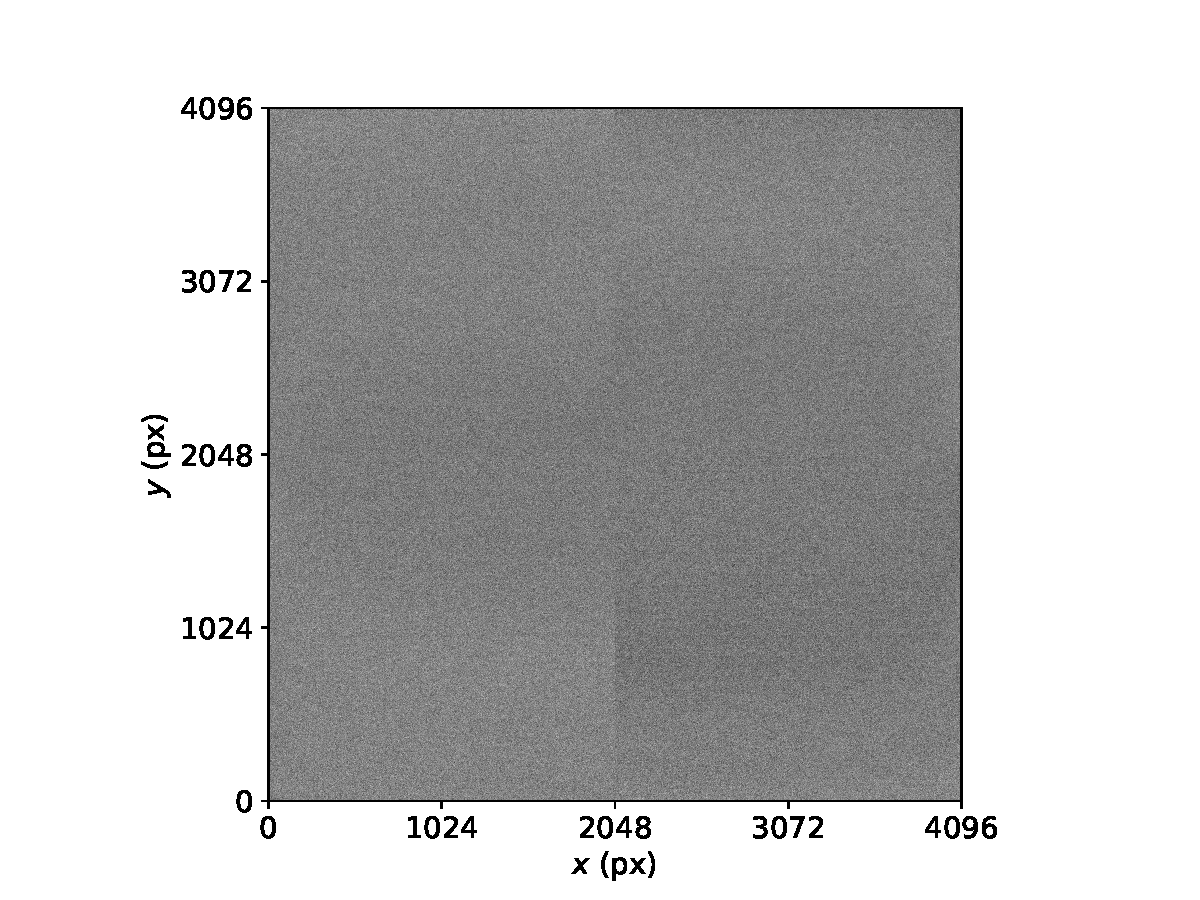
\includegraphics[width=0.7\columnwidth]{figures/dark-60-diff.pdf}
\medskip
\caption{Difference between the residual bias images formed the last and first images in 280 sequences of 5 dark images with exposure times of 60 seconds. The gray scale is $(-1,+1)$ DN.}
\label{figure:dark-60-diff}
\end{center}
\end{figure}

\begin{figure}[pb]
\begin{center}
\includegraphics[width=0.7\columnwidth]{figures/dark-60-diff-y.pdf}
\medskip
\caption{The mean values in the $x$ direction of the difference between the residual bias images formed the last and first images in 280 sequences of 5 dark images with exposure times of 60 seconds.}
\label{figure:dark-60-diff-y}
\end{center}
\begin{center}
\includegraphics[width=0.7\columnwidth]{figures/dark-60-diff-x.pdf}
\medskip
\caption{The mean values in the $y$ direction of the difference between the residual bias images formed the last and first images in 280 sequences of 5 dark images with exposure times of 60 seconds.}
\label{figure:dark-60-diff-x}
\end{center}
\end{figure}

We also took 280 sequences of 5 darks with exposure times of 60 seconds. At $-110$~C, the typical dark current of these CCDs is 0.25 electrons per pixel per hour, so the accumulated dark current in these exposures is expected to be typically 0.004 electrons or 0.002 DN. This is completely negligible. For most purposes, these dark images are equivalent to biases but with a delay of 60 seconds between the reset and the read. Figure~\ref{figure:dark-60-residual-sequence} shows the mean values of the residual in each quadrant as a function of the index in the sequence of 5 darks. The curves for the darks are much flatter than for the biases. Also, the values of the curves for the darks are fairly close to the values for the initial biases.

Figures~\ref{figure:dark-60-a} and \ref{figure:dark-60-b} show residual bias images formed from the first and last images in sequences of 5 dark images. We note that the gradients seen in quadrants 2 and 4 in these images are almost certainly not the result of dark current, since they are too large (roughly $\pm1$ DN) and are not seen in quadrants 1 and 4. We would suggest from their form that they might be due to spurious charge. Figure~\ref{figure:dark-60-diff} shows the difference between the residual bias images. Figures~\ref{figure:dark-60-diff-y} and \ref{figure:dark-60-diff-x} show the means in the difference images in the $x$ and $y$ directions. Comparing these to the equivalents for the images formed from the bias sequences, we see that the changes are much smaller, roughly $\pm0.1$ DN compared to $\pm0.5$ DN. 

It would seem that taking biases in rapid succession perturbs the residual values. In both the bias and dark sequences, the resets follow rapidly after the preceding read. However, in the bias sequences the reads follow rapidly after the preceding resets whereas in the dark sequences the reads occur 60 seconds after the preceding resets. Thus, the problem seems to be when reads rapidly follow resets.

The data suggest that a delay of 60 seconds is long enough to avoid this phenomenon. However, we do not have data that would allow us to explore whether shorter delays might also give benign behavior; this is something that should be investigated in the future.

This phenomenon has a couple of implications. First, we need to note that these effects are only seen at the $\pm1$ electron level and so will be negligible in many applications. However, the uncertainty in the bias level will make it difficult to determine the dark current with precision, as this is expected to be at the level of about 0.25 electron or 0.1 DN per hour. Second, we would recommend that rather than subtracting a residual bias image (with 0 seconds of exposure) and a scale dark image, it is probably safer to subtract a combined bias and dark image with an similar exposure time. This approach is common in infrared instruments. 

For the rest of the analysis presented here, we will use a residual bias formed from darks with exposure times of 60 seconds, unless we explicitly state otherwise.

\clearpage
\section{Instrument Background}

\begin{figure}[pb]
\begin{center}
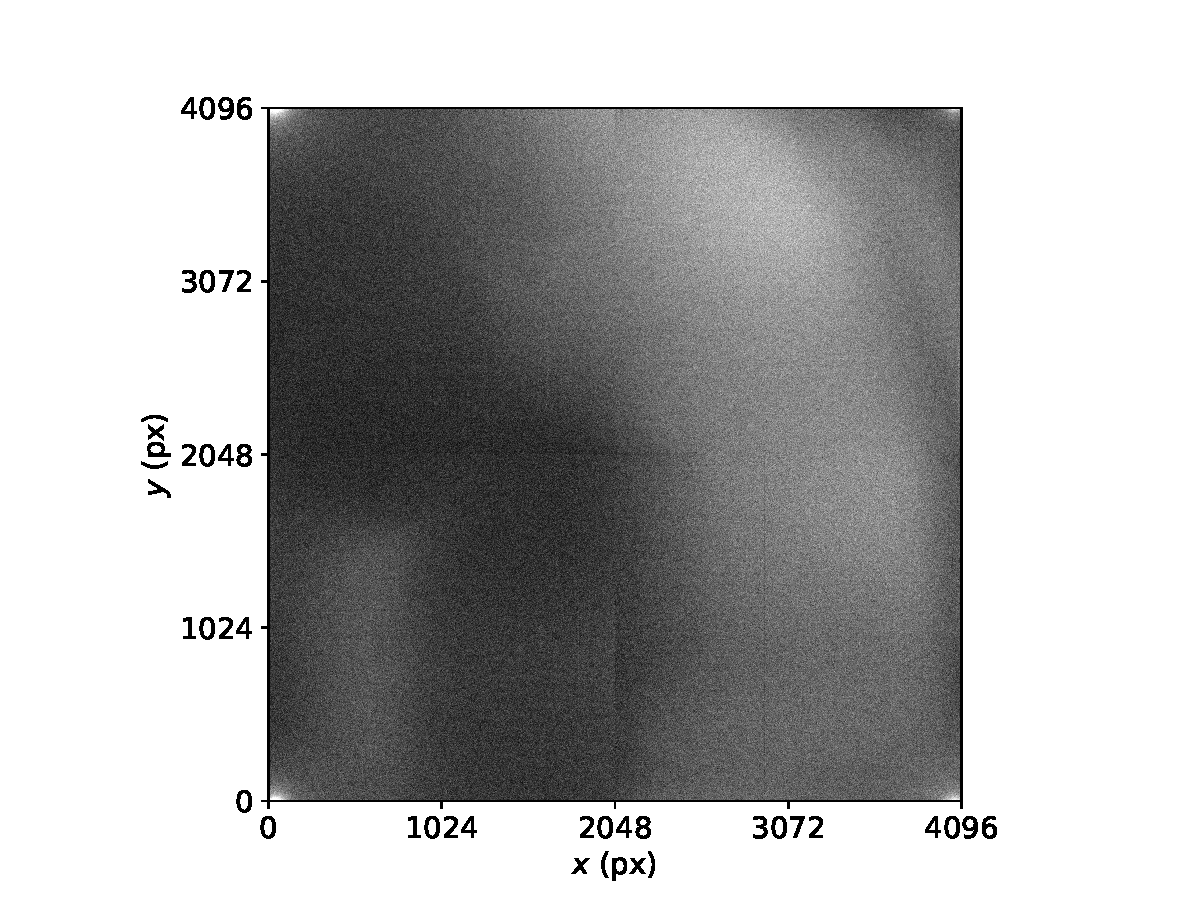
\includegraphics[width=0.7\columnwidth]{figures/dark-600.pdf}
\medskip
\caption{Instrument background image formed from 260 dark images with exposure times of 600 seconds. The gray scale is $(0,2)$ DN.}
\label{figure:dark-600}
\end{center}
\end{figure}

\begin{figure}[pb]
\begin{center}
\includegraphics[width=0.7\columnwidth]{figures/dark-600-y.pdf}
\medskip
\caption{The mean values in the $x$ direction of the instrument background image formed from 260 dark images with exposure times of 600 seconds.}
\label{figure:dark-600-y}
\end{center}
\begin{center}
\includegraphics[width=0.7\columnwidth]{figures/dark-600-x.pdf}
\medskip
\caption{The mean values in the $y$ direction of the instrument background image formed from 260 dark images with exposure times of 600 seconds.}
\label{figure:dark-600-x}
\end{center}
\end{figure}

\begin{figure}[pb]
\begin{center}
\includegraphics[width=0.7\columnwidth]{figures/dark-600-time.pdf}
\medskip
\caption{The mean values in the dark images with exposure times of 600 seconds and the moon illumination fraction during commissioning. The mean level tracks the illumination of the moon, which suggests we are seeing the result of ambient light leaking around the shutter.}
\label{figure:dark-600-time}
\end{center}
\end{figure}

Along with the sequences of 10 biases and 5 darks with exposure times of 60 seconds, we also took about 260 dark images with exposure times of 600 seconds. We used these to form images of the instrument background (after subtracting the underscan level and residual bias). 

Figure~\ref{figure:dark-600} shows the instrument background image formed from these images. Figures~\ref{figure:dark-60-diff-y} and \ref{figure:dark-60-diff-x} show the means in the images in the $x$ and $y$ directions.

In this image we propose that we are mainly seeing light leaking around the shutter. The reasons are multiple. First, the pattern seems similar to images we have seen in the laboratory with clear light leaks. Second, the spatial scale is appropriate for light leaks but not for dark current. Third, the level (about 1 DN in 600 seconds or 12 electrons per hour per pixel) is much larger than the dark current expected for the detector. Finally, as Figure~\ref{figure:dark-600-time} shows, we see the level vary by about a factor of two over the run and this change tracks the illumination of the Moon.

However, we also see what appears to be amplifier glow in the corners at the level of about 1 DN in 600 seconds or, again, about 12 electrons per hour per pixel.

The lowest expected sky background is about 1 electron per pixel per second when using $B$ in dark time \cite{expected}. Thus, both the light leak and the amplifier glow are about 1/300 of this background. Nevertheless, while this level of instrument background is well within specification, we will attempt to reduce it further in DDRAGO.

\clearpage
\section{Read-Noise}

\begin{figure}[pb]
\begin{center}
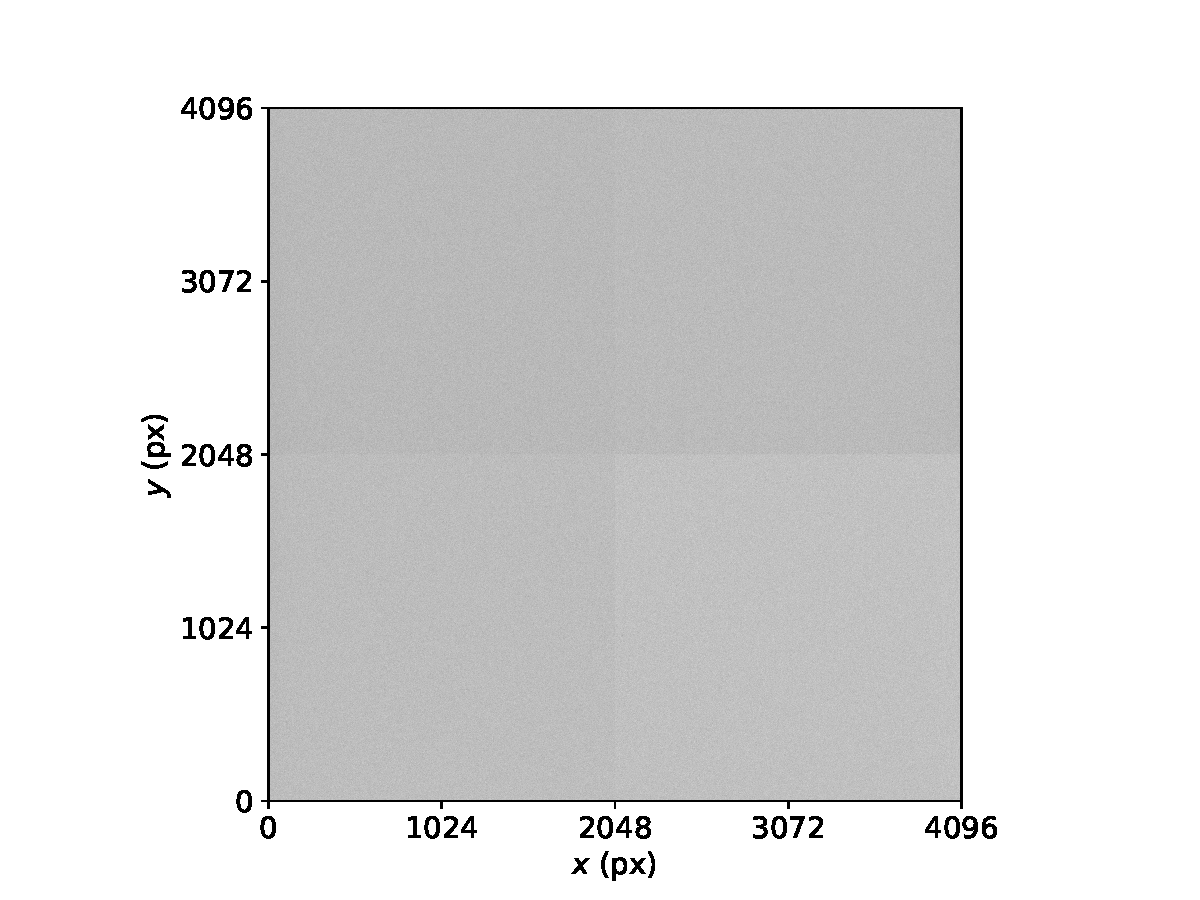
\includegraphics[width=0.7\columnwidth]{figures/read-noise.pdf}
\medskip
\caption{Read-noise image formed from 256 bias images. The gray scale is $(0,4)$ DN.}
\label{figure:read-noise}
\end{center}
\end{figure}

\begin{figure}[pb]
\begin{center}
\includegraphics[width=0.7\columnwidth]{figures/read-noise-y.pdf}
\medskip
\caption{The mean values in the $x$ direction of the read-noise image formed from 256 bias images.}
\label{figure:read-noise-y}
\end{center}
\begin{center}
\includegraphics[width=0.7\columnwidth]{figures/read-noise-x.pdf}
\medskip
\caption{The mean values in the $y$ direction of the read-noise image formed from 256 bias images.}
\label{figure:read-noise-x}
\end{center}
\end{figure}

\begin{table}[pb]
\begin{center}
\caption{Measured Read-Noise (DN)}
\label{table:read-noise}
\begin{tabular}{ccc}
\hline
Quadrant&Laboratory&Commissioning\\
\hline
0&2.97&2.95\\
1&3.05&3.02\\
2&2.90&2.89\\
3&2.95&2.92\\
\hline
\end{tabular}
\end{center}
\end{table}

\begin{figure}[pb]
\begin{center}
\includegraphics[width=0.7\columnwidth]{figures/read-noise-azimuth.pdf}
\medskip
\caption{The read-noise as a function of azimuth.}
\label{figure:read-noise-azimuth}
\end{center}
\end{figure}

\begin{figure}[pb]
\begin{center}
\includegraphics[width=0.7\columnwidth]{figures/read-noise-time.pdf}
\medskip
\caption{The read-noise during commissioning.}
\label{figure:read-noise-time}
\end{center}
\end{figure}

At first sight, the variation in the bias level discussed above complicates the estimation of the read-noise. However, the read-noise is expected to be about 3 DN and the variations are at the level of a fraction of a DN. Therefore, the actual quantitative impact of the variation on measurements of the read-noise is negligible.

During the commissioning we took about 2800 bias images. Figure~\ref{figure:read-noise} shows the read-noise image formed from 256 of these images. Figures~\ref{figure:read-noise-y} and \ref{figure:read-noise-x} show the means in the read-noise image in the $x$ and $y$ directions. Each quadrant has a slightly different read-noise (as expected as each quadrant has a different amplifier). There is quadrants are largely uniform, with slight structure at the top and bottom that may be related to the variations in the bias (cf. Figure~\ref{figure:bias-diff-x}).

On 2023 March 17 we took 5 biases at azimuths of $0$, $45$, $90$, \ldots, $315$ degrees and a zenith distance of 45 degrees. Figure~\ref{figure:read-noise-azimuth} shows the dependence of the read-noise on azimuth. The variations are small.

Figure~\ref{figure:read-noise-time} shows the read-noise calculated each night during commissioning. Again, the variations are small.

Table~\ref{table:read-noise} shows the read-noise measured in the laboratory tests \cite{laboratory} and during commissioning. They are essentially identical. We did not measure the gain during commissioning, but in the laboratory it was found to be 2.23 electrons for the read-mode used during commissioning and essentially uniform between quadrants. Thus, the read-noises measured during commissioning correspond to 6.4--6.7 electrons.

We conclude that the read-noise values are very similar to those measured in the laboratory and that variations with time and position during commissioning are small.

\clearpage
\section{Flat Fields}

\begin{figure}[pb]
\begin{center}
\includegraphics[width=0.7\columnwidth]{figures/flat-g-20230317.pdf}
\medskip
\caption{The $g$ flat from 2023-03-17. The gray scale is $(0,1.25)$.}
\label{figure:flat-g-20230317}
\end{center}
\end{figure}

\begin{figure}[pb]
\begin{center}
\includegraphics[width=0.7\columnwidth]{figures/flat-g-20230328.pdf}
\medskip
\caption{The $g$ flat from 2023-03-28. The gray scale is $(0,1.25)$.}
\label{figure:flat-g-20230328}
\end{center}
\end{figure}

\begin{figure}[pb]
\begin{center}
\includegraphics[width=0.7\columnwidth]{figures/flat-g-20230329.pdf}
\medskip
\caption{The $g$ flat from 2023-03-29. The gray scale is $(0,1.25)$.}
\label{figure:flat-g-20230329}
\end{center}
\end{figure}

\begin{figure}[pb]
\begin{center}
\includegraphics[width=0.7\columnwidth]{figures/flat-r-20230328.pdf}
\medskip
\caption{The $r$ flat from 2023-03-28. The gray scale is $(0,1.25)$.}
\label{figure:flat-r-20230328}
\label{figure:flat-first}
\end{center}
\end{figure}

\begin{figure}[pb]
\begin{center}
\includegraphics[width=0.7\columnwidth]{figures/flat-i-20230315.pdf}
\medskip
\caption{The $i$ flat from 2023-03-15. The gray scale is $(0,1.25)$.}
\label{figure:flat-i-20230315}
\end{center}
\end{figure}

\begin{figure}[pb]
\begin{center}
\includegraphics[width=0.7\columnwidth]{figures/flat-i-20230329.pdf}
\medskip
\caption{The $i$ flat from 2023-03-29. The gray scale is $(0,1.25)$.}
\label{figure:flat-i-20230329}
\end{center}
\end{figure}

\begin{figure}[pb]
\begin{center}
\includegraphics[width=0.7\columnwidth]{figures/flat-z-20230315.pdf}
\medskip
\caption{The $z$ flat from 2023-03-15. The gray scale is $(0,1.25)$.}
\label{figure:flat-z-20230315}
\end{center}
\end{figure}

\begin{figure}[pb]
\begin{center}
\includegraphics[width=0.7\columnwidth]{figures/flat-z-20230329.pdf}
\medskip
\caption{The $z$ flat from 2023-03-29. The gray scale is $(0,1.25)$.}
\label{figure:flat-z-20230329}
\end{center}
\end{figure}

\begin{figure}[pb]
\begin{center}
\includegraphics[width=0.7\columnwidth]{figures/flat-y-20230315.pdf}
\medskip
\caption{The $y$ flat from 2023-03-15. The gray scale is $(0,1.25)$.}
\label{figure:flat-y-20230315}
\end{center}
\end{figure}

\begin{figure}[pb]
\begin{center}
\includegraphics[width=0.7\columnwidth]{figures/flat-y-20230329.pdf}
\medskip
\caption{The $y$ flat from 2023-03-29. The gray scale is $(0,1.25)$.}
\label{figure:flat-y-20230329}
\label{figure:flat-last}
\end{center}
\end{figure}

\begin{figure}[pb]
\begin{center}
\includegraphics[width=0.7\columnwidth]{figures/flat-vignetting.pdf}
\medskip
\caption{The vignetting in the $i$ flat from 2023-03-15. The radius is referred to the detector center. The solid vertical line marks the inscribed field and the dotted vertical line marks a field with a diameter of 2200 pixels.}
\label{figure:flat-vignetting}
\end{center}
\end{figure}

\begin{figure}[pb]
\begin{center}
\includegraphics[width=0.7\columnwidth]{figures/flat-vignetting-shifted.pdf}
\medskip
\caption{The vignetting in the $i$ flat from 2023-03-15. The radius is referred to a point shifted $+70$ pixels in $x$ and $+10$ pixels in $y$ from the detector center. The solid vertical line marks the inscribed field and the dotted vertical line marks a field with a diameter of 2200 pixels.}
\label{figure:flat-vignetting-shifted}
\end{center}
\end{figure}

\begin{figure}[pb]
\begin{center}
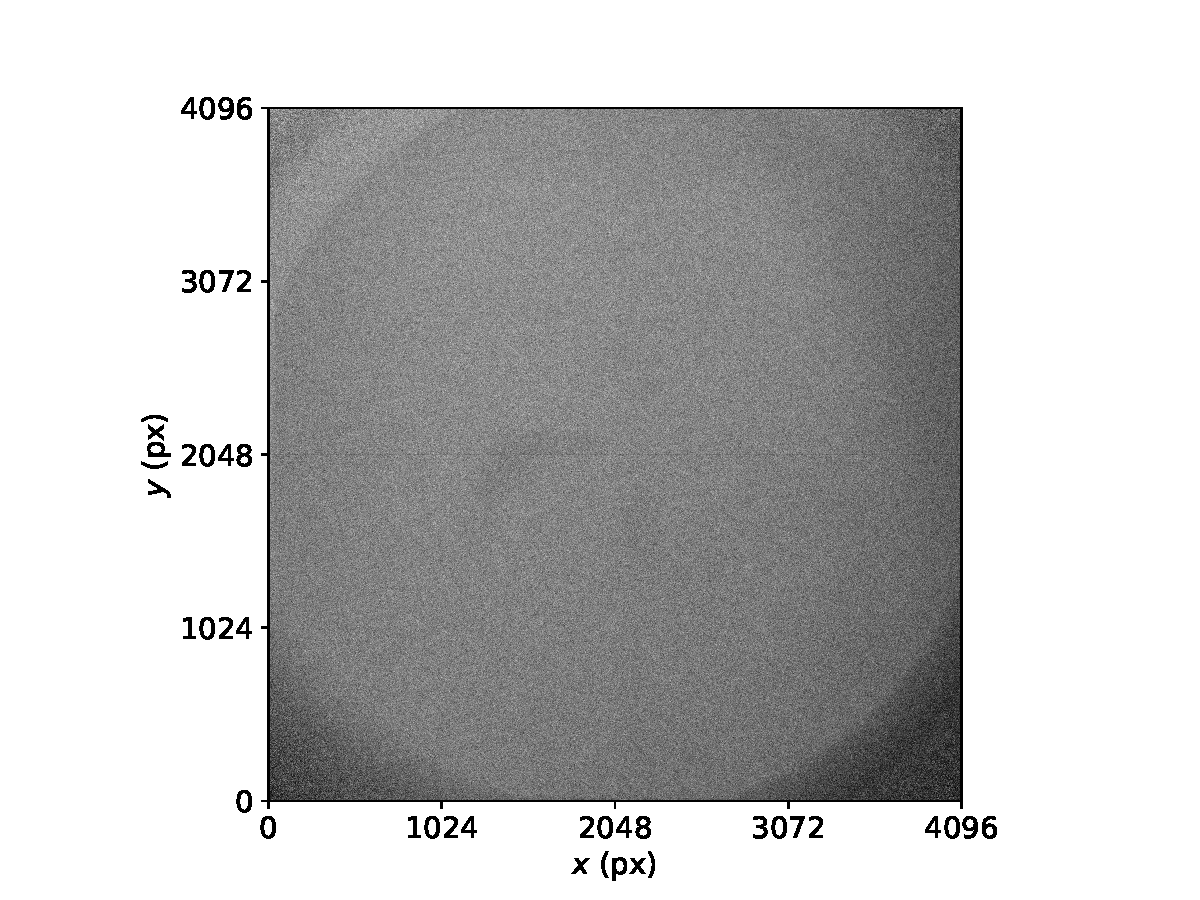
\includegraphics[width=0.48\columnwidth]{figures/flat-ratio-g-20230317-g-20230328-hard.pdf}
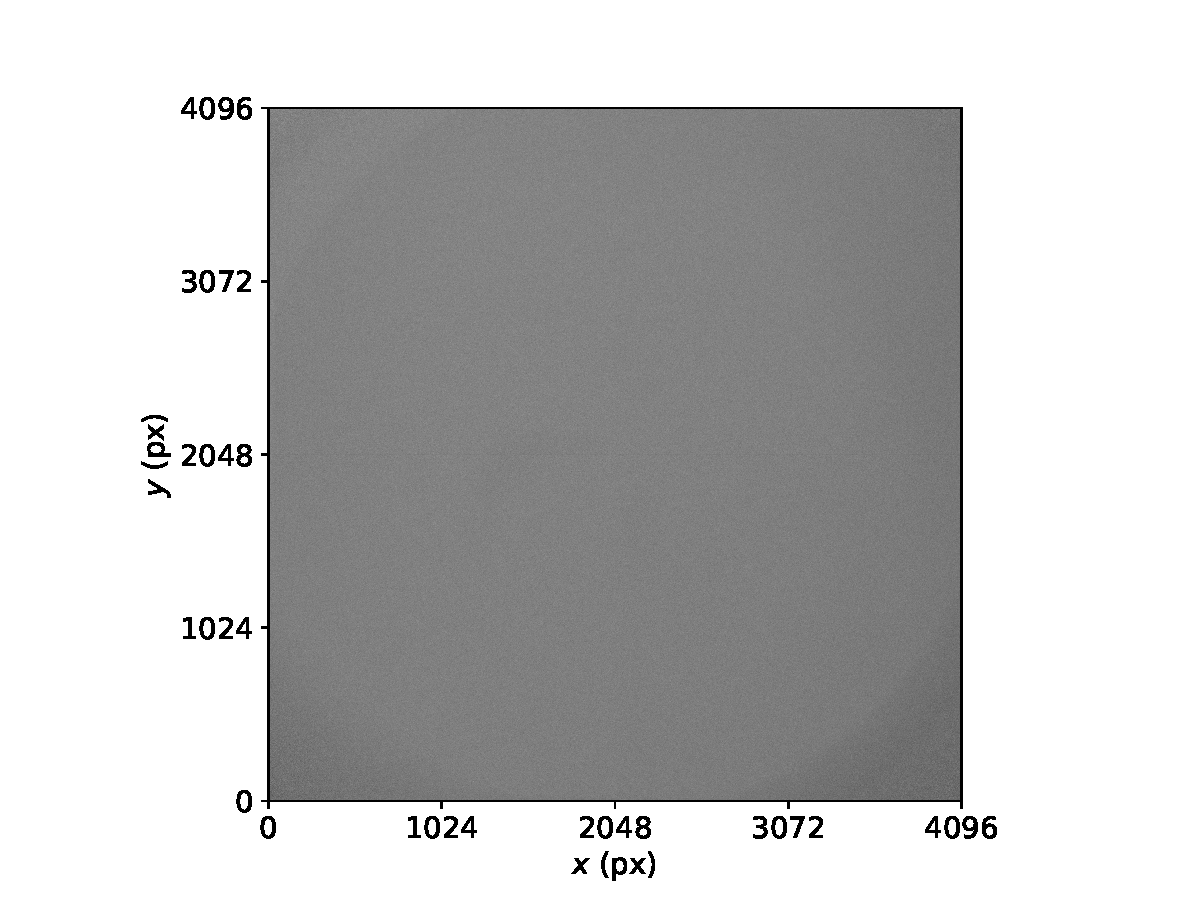
\includegraphics[width=0.48\columnwidth]{figures/flat-ratio-g-20230317-g-20230328-soft.pdf}
\medskip
\caption{The ratio between in the $g$ flats from 2023-03-17 and 2023-03-28. The gray scales are (0.99,1.01) and (0.96,1.04).}
\label{figure:flat-ratio-g-20230317-g-20230328}
\label{figure:flat-ratio-first}
\end{center}
\end{figure}

\begin{figure}[pb]
\begin{center}
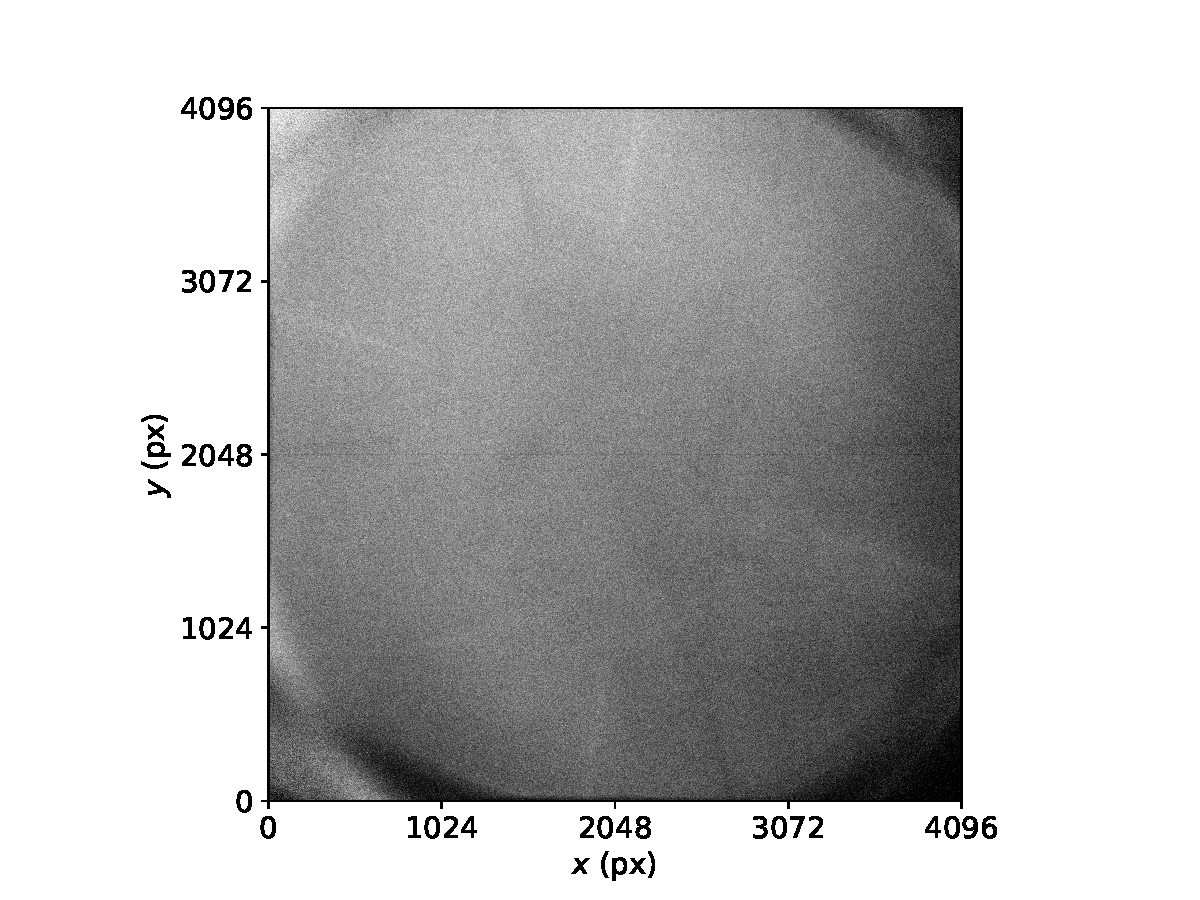
\includegraphics[width=0.48\columnwidth]{figures/flat-ratio-g-20230317-g-20230329-hard.pdf}
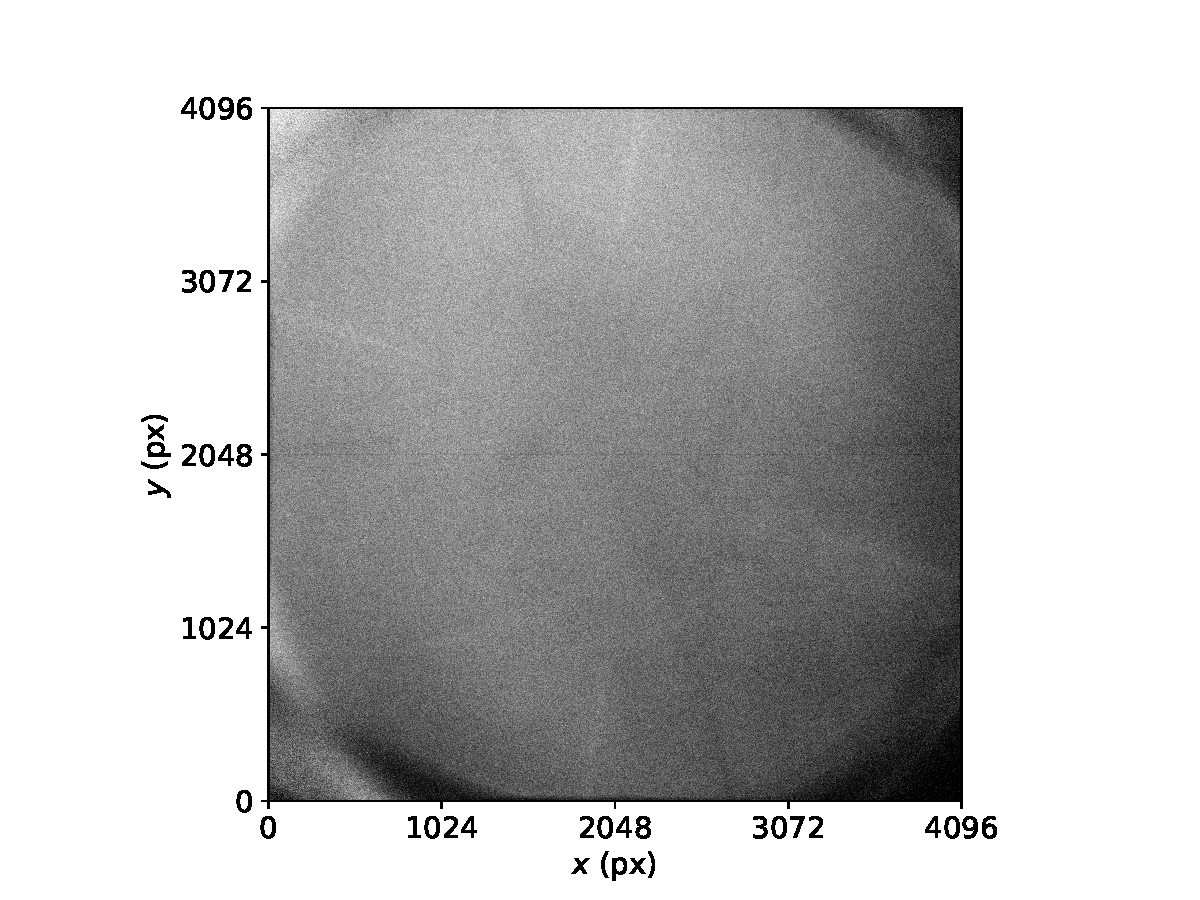
\includegraphics[width=0.48\columnwidth]{figures/flat-ratio-g-20230317-g-20230329-hard.pdf}
\medskip
\caption{The ratio between in the $g$ flats from 2023-03-17 and 2023-03-29. The gray scales are (0.99,1.01) and (0.96,1.04).}
\label{figure:flat-ratio-g-20230317-g-20230329}
\end{center}
\end{figure}

\begin{figure}[pb]
\begin{center}
\includegraphics[width=0.48\columnwidth]{figures/flat-ratio-g-20230328-g-20230329-hard.pdf}
\includegraphics[width=0.48\columnwidth]{figures/flat-ratio-g-20230328-g-20230329-soft.pdf}
\medskip
\caption{The ratio between in the $g$ flats from 2023-03-28 and 2023-03-29. The gray scales are (0.99,1.01) and (0.96,1.04).}
\label{figure:flat-ratio-g-20230328-g-20230329}
\end{center}
\end{figure}

\begin{figure}[pb]
\begin{center}
\includegraphics[width=0.48\columnwidth]{figures/flat-ratio-i-20230315-i-20230329-hard.pdf}
\includegraphics[width=0.48\columnwidth]{figures/flat-ratio-i-20230315-i-20230329-soft.pdf}
\medskip
\caption{The ratio between in the $i$ flats from 2023-03-15 and 2023-03-29. The gray scales are (0.99,1.01) and (0.96,1.04).}
\label{figure:flat-ratio-i-20230315-i-20230329}
\end{center}
\end{figure}

\begin{figure}[pb]
\begin{center}
\includegraphics[width=0.48\columnwidth]{figures/flat-ratio-z-20230315-z-20230329-hard.pdf}
\includegraphics[width=0.48\columnwidth]{figures/flat-ratio-z-20230315-z-20230329-soft.pdf}
\medskip
\caption{The ratio between in the $z$ flats from 2023-03-15 and 2023-03-29. The gray scales are (0.99,1.01) and (0.96,1.04).}
\label{figure:flat-ratio-z-20230315-z-20230329}
\end{center}
\end{figure}

\begin{figure}[pb]
\begin{center}
\includegraphics[width=0.48\columnwidth]{figures/flat-ratio-y-20230315-y-20230329-hard.pdf}
\includegraphics[width=0.48\columnwidth]{figures/flat-ratio-y-20230315-y-20230329-soft.pdf}
\medskip
\caption{The ratio between in the $y$ flats from 2023-03-15 and 2023-03-29. The gray scales are (0.99,1.01) and (0.96,1.04).}
\label{figure:flat-ratio-y-20230315-y-20230329}
\label{figure:flat-ratio-last}
\end{center}
\end{figure}

\begin{table}[pb]
\begin{center}
\caption{Statistics of Ratios of Flats}
\label{table:flat-ratio}
\footnotesize
\begin{tabular}{ccccccccc}
\hline
Filter&Date&Date&\multicolumn{3}{c}{Inside Inscribed}&\multicolumn{3}{c}{Outside Inscribed}\\
&&&$\sigma$&1\%&99\%&$\sigma$&1\%&99\%\\
\hline
$g$ & 2023-03-17 & 2023-03-28 & 0.003 & $-0.007$ & $+0.007$ & 0.004 & $-0.011$ & $+0.007$ \\
$g$ & 2023-03-17 & 2023-03-29 & 0.004 & $-0.008$ & $+0.008$ & 0.005 & $-0.015$ & $+0.009$ \\
$g$ & 2023-03-28 & 2023-03-29 & 0.003 & $-0.007$ & $+0.007$ & 0.004 & $-0.010$ & $+0.009$ \\
$i$ & 2023-03-15 & 2023-03-29 & 0.003 & $-0.008$ & $+0.008$ & 0.010 & $-0.017$ & $+0.035$ \\
$z$ & 2023-03-15 & 2023-03-29 & 0.003 & $-0.008$ & $+0.008$ & 0.012 & $-0.028$ & $+0.040$ \\
$y$ & 2023-03-15 & 2023-03-29 & 0.006 & $-0.014$ & $+0.014$ & 0.009 & $-0.012$ & $+0.037$ \\
\hline
\end{tabular}
\end{center}
\end{table}

We took flat fields on several nights. We constructed flat field images for those nights for which we have at least five images with mean level in the inscribed circle of between 10,000 and 30,000 DN (so the SNR is at least 150 in each image). The flats are constructed by normalizing to the mean level in the inscribed circle and then averaging with $2\sigma$ rejection.

We have three flats in $g$ (from 2023-03-17, 2023-03-28, and 2023-03-29), one flat in $r$ (from 2023-03-28), two flats in $i$ (from 2023-03-15 and 2023-03-29), two flats in $z$ (from 2023-03-15 and 2023-03-29), and two flats in $y$ (from 2023-03-15 and 2023-03-29). They are shown in Figures~\ref{figure:flat-first} to \ref{figure:flat-last}.

Figure~\ref{figure:flat-vignetting} shows that the flats have essentially no vignetting in a field of about 2200 pixels (14.0 arcmin) in radius, slightly larger than the inscribed circle, but strong vignetting in the corners. The vignetting pattern is not perfectly centered on the detector, but is shifted by about $+70$ pixels in $x$ and $+10$ pixels in $y$. Figure~\ref{figure:flat-vignetting-shifted} shows the vignetting with respect to this center. This degree of vignetting in the corners was \emph{not} predicted in the design. We are currently investigating its origin.

The flats show other features. In all, there is a large donut in the lower right with an amplitude of about 2\%. The $g$ flats (only) show diagonal stripes, possibly a feature in the substrare. The $y$ flats show a linear or rectangular feature on the right.

Figures~\ref{figure:flat-ratio-first} to \ref{figure:flat-ratio-last} show ratios of flats taken in the same filters on different nights. The stretches are $\pm1\%$ and $\pm4\%$. To understand these, it is important to note that the flats from 2023-03-15 to 2023-03-28 were taken at the same derotator angle, but the flats on 2023-03-29 were taken at a different derotator angle.

We will divide the discussion into two parts: the behavior in the unvigenetted region (which is slightly larger than the inscribed) circle and the behavior in the vignetted region. The statistics of these two ratios in these two regions (standard deviations and 1\%-ile, and 99\%-ile deviations from the mean) are shown in Table~\ref{table:flat-ratio}.

We first consider the ratio of the $g$ flats taken on 2023-03-17 and 2023-03-28, shown in Figure~\ref{figure:flat-ratio-g-20230317-g-20230328}. These two flats were taken with the same derotator position. The ratio is almost perfectly flat in the unvignetted region, with just a low contrast arc-shaped feature, the standard deviation is $0.003$ and the 1\%-ile and 99\%-ile are $\pm0.007$ from the mean. The diagonal stripes seen in the flat fields disappear in the ratio. Outside of the unvignetted region, the deviations are slightly larger and we see a systematic pattern that appears to correspond to the vignetting pattern moving vertically with respect to the detector (or vice versa).

The appearance in the flats of features corresponding to the secondary and tertiary supports is actually quite easy to understand. At the field center, the secondary and tertiary supports coincide in the pupil and the geometric transmission is maximized. At most points in the field, the supports will not coincide in the pupil and the geometric transmission is minimized. However, at position angles that correspond to one of the supports, two of the supports coincide and two do not, so the geometric transmission is between these two extrema.

We next consider the ratio of the $g$ flats taken on 2023-03-17 and 2023-03-29, shown in Figure~\ref{figure:flat-ratio-g-20230317-g-20230328}. These two flats were taken at different derotator positions. In the unvignetted region, the raw statistics are only slightly worse, with the standard deviation being 0.004 and the 1\%-ile and 9\%-ile deviations being $\pm0.008$. Nevertheless, we see significantly more structure in the ratio in the form of arcs and, apparently, the pattern of the secondary supports. Outside of the unvignetted region, the statistics are slightly worse and again we see a pattern that appears to result from a shift of the vignetting to the upper left.

We see similar results in the ratios of the $i$, $z$, and $y$ flats taken on 2023-03-15 and 2023-03-29, shown in Figures~\ref{figure:flat-ratio-i-20230315-i-20230329}, \ref{figure:flat-ratio-z-20230315-z-20230329}, and \ref{figure:flat-ratio-y-20230315-y-20230329}, except that the vignetting pattern seems to have shifted to the left. Furthermore, outside the vignetted region in these ratios the deviations are much larger, with standard deviations being $0.009$--$0.012$ and the 1\%-ile and 99\%-ile deviations being as large as 0.040.

Finally, in the ratio of the $y$ flats taken on 2023-03-15 and 2023-03-29, shown in Figure~\ref{figure:flat-ratio-y-20230315-y-20230329}, we see that the linear feature has moved. We suspect that this feature might be related to the filter holder or the filter wheel, since these are the only non-circular elements in the optical beam. We will examine the filter wheel when it is returned to Mexico. In this ratio, we also see evidence for different fringes in the two flats, but at a low level.

In summary, we find that the detector is unvignetted out to a diameter of about 2200 pixels. In the unvignetted region, the flats have structure that changes with the derotator position but this structure is at a level of less than 1\%. Outside of the unvignetted region, the flats vary by up to several percent.

The variability of the flat outside of the unvignetted region has two implications. One is that conventional photometry here will have uncertainties of several percent. The other is that we expect the sky level to vary by this much as the derotator rotates. Thus, in order to obtain sensitivity below the level of the sky, we will need to form sky flats from images at similar derotator angles.

We have at least three tasks in hand. The first is to understand the origin of the vignetting; we repeat that it was not predicted in the optical design study. The second is to understand (in DDRAGO on the telescope) its dependency on derotator angle or other variables. If the variance is relatively reproducible, we might be able to build a library of flats and apply them appropriately to science images. The last is to understand the linear feature in the $y$ flats.

\clearpage
\section{Scale and Distortion}

We measured the scale and distortion by running astrometry.net on the first images in each filter for the block 0005/7 on 2023 March 20. We then used the solution to determine the scale at the center of the detector, the range of linear scales in $x$ and $y$, and the range of pixel areas. These are shown in Table~\ref{table:scale}. The ranges are given as the minimum and maximum fractional deviations.

\begin{table}[pb]
\begin{center}
\caption{Scale and Distortion}
\label{table:scale}
\begin{tabular}{cccc}
\hline
Filter&Center Scale&Scale Range&Area Range\\
\hline
$g$ & 0.3789 & $-00006$ to $+0.0006$ & $-0.0010$ to $+0.0009$ \\
$r$ & 0.3790 & $-00005$ to $+0.0004$ & $-0.0008$ to $+0.0008$ \\
$i$ & 0.3790 & $-00008$ to $+0.0007$ & $-0.0015$ to $+0.0014$ \\
$z$ & 0.3789 & $-00004$ to $+0.0004$ & $-0.0007$ to $+0.0006$ \\
$y$ & 0.3789 & $-00005$ to $+0.0003$ & $-0.0008$ to $+0.0007$ \\
\hline
\end{tabular}
\end{center}
\end{table}

The central scale is 0.379 arcsec per pixel and is uniform with wavelength to within 0.1 milliarcsec. The largest fractional linear distortion is $\pm 0.0008$ (i.e., less than 1 part in 1000) and the largest fractional area distortion is $\pm0.0015$ (i.e., slightly larger than 1 part in 1000).

The requirement is that the distortion be less than 5\%, so we satisfy this by about a factor of 60.

The main implication of this is that we do not need to worry unduly about the difference between areal photometry and point-source photometry, since the pixel area changes by only about $\pm0.1\%$ over the field.

\clearpage
\section{Zero-Points}

We measured the zero points using aperture photometry on the images in each filter for the block 0005/7 on 2023 March 20. These images were taken at airmasses of 1.01 to 1.12. We used an aperture with a radius of 10 pixels. We compared the measured signals to the PS1 DR2 photometry, assuming a gain of 2.23 electrons per DN, and fitting for a linear color term in $g-r$. Table~\ref{table:zero-points} shows the model \cite{expected} and measured zero-points in electrons per second and their ratio. (The model zero-points are for DDRAGO at OAN at an airmass of 1.5.)

We see that the zero points are lower than expected by factors of 2.5 to 4. Some of this is probably due to the poor state of the mirrors and perhaps the higher atmospheric extinction at OHP.

\begin{table}[pb]
\begin{center}
\caption{Zero-Points}
\label{table:zero-points}
\begin{tabular}{cccc}
\hline
Filter&Model&Measured& Ratio\\
\hline
$g$  &$5.24 \times 10^{9}$ & $1.36 \times 10^{9}$ & 0.26\\
$r$  &$4.34 \times 10^{9}$ & $1.67 \times 10^{9}$ & 0.38\\
$i$  &$3.25 \times 10^{9}$ & $1.19 \times 10^{9}$ & 0.37\\
$z$  &$1.71 \times 10^{9}$ & $6.01 \times 10^{8}$ & 0.35\\
$y$  &$6.85 \times 10^{8}$ & $2.09 \times 10^{8}$ & 0.31\\
\hline
\end{tabular}
\end{center}
\end{table}

\clearpage
\section{Charge-Transfer Efficiency}

\clearpage
\section{Summary}

DDRAGUITO was commissioned on the COLIBRI telescope at OHP in 2023 March and April. In this document, we have analysed the data. We conclude:

\begin{enumerate}

\item The detector was able to achieve its working temperature of $-110$~C. However, there were periods in which it was not able to maintain this temperature. These periods corresponded to cold nights, with temperatures well below the stated operating temperature range of the service cabinet. Furthermore, we were not able to recharge the cryogen to full pressure. In OHP, the service cabinet was exposed to outside temperatures. At OAN, it will be operated in a temperature-controlled environment and should be charged to full pressure. Nevertheless, we need to verify that the system is able to maintain a stable temperature at OAN.

\item Before cooling-down, we pumped-down the chamber from 0.3 to 0.01~mbar. After warming-up, the pressure had rebounded to 0.2 mbar. This suggests that we need to be ready to pump-down the chamber at OAN.

\item The detector underscan varies and should be calculated and subtracted from each quadrant.

\item The residual bias shows shows structure that depends on the read-out history and has variations at the level of 0.3 DN. Instead of taking conventional biases, we recommend taking darks with the same (or similar) exposure time as object frames and subtracting these.

\item The instrument background was dominated by ambient moonlight leaking around the shutter and amplifier glow, both or which were observed to be about 12 electrons per pixel per hour. This is a factor of 300 less than the lowest expected sky background.

\item The read-noise was measured to be about 6.5 electrons. We found no evidence of significant variances with time or position.

\item The field is essentially unvignetted to a radius of 2200 pixels. Beyond this, there is severe vignetting and in the corners of the detector the transmission is only about 40\% of that in the unvignetted region. The flat fields in the unvignetted region are consistent to better than 1\%. However, in the vignetted region they vary by several percent, apparently with the derotator angle. 

\item In the ratio of the $y$ flats we see a linear feature with a contrast of about 2\% that might be related to the filter or filter wheel. This feature requires further investigation.

\item The scale in the center of the detector is $0.3790$ arcsec per pixel and varies between filters by only 1 part in 10,000 and over the field by only 1 part in 1000.

\item The zero-points are lower than the model for DDRAGO at OAN. Some of this may be due to the poor state of the mirrors and the higher extinction at OHP.
\end{enumerate}



\clearpage
\begin{thebibliography}{Te2v}

\bibitem{optical-design}
“COLIBRÍ Optical Design,” Jorge Fuentes, Alan Watson, \& Salvador Cuevas, 2022 March 9, COLIBRI-UNAM-DS-1, Version 8.2

\bibitem{laboratory}
“DDRAGUITO: Detector and Filter Wheel Laboratory Verification,” Alan Watson, 2020 November 12, Version 1.0.

\bibitem{expected}
“COLIBRI Expected Performance,” Alan Watson, 2018 May 9, GFT-AN-A3135-046-UNAM, Version 2.1

\bibitem{dolon}
“DDRAGUITO integration at OHP,” François Dolon, 2023 April 19, COLIBRI OHP Note 10, Edition 1, Revision 2.

\bibitem{service-cabinet}
“Series 1100/1110 Camera System Service Cabinet Modular Version Service Manual,” Spectral Instruments, 2014 March 31

\bibitem{e2v}
“CCD231-84 Back-illuminated Scientific Sensor,” Teledyne e2v, August 2018, A1A-765136 Version 8

\end{thebibliography}

\clearpage
\appendix
\section{Contemporaneous Notes}
\label{appendix:notes}

This section contains the contemporaneous notes taken by Alan Watson during the commissioning run. They are a guide to what data was taken when and for what purpose.

These notes assume that the filter order was $rgizy$. We now believe that the filter order was $grizy$. Thus, we believe that all references to $g$ in these notes are actually references to $r$ and all references to $r$ are actually references to $g$.

\subsection{2023-03-13}

François filled to 221 PSI.

\subsection{2023-03-14 Day}

François (local) and Alan (remote)

While disconnecting the bottle, there was a leak and the pressure dropped from 221 PSI to 178 PSI. The bottle no longer seems to have any pressure (François says that the valve on the refill hose is at 0). We decided to cool. The detector cooled to $-110$~C in just under three hours and was stable for the following 24 hours.

\subsection{2023-03-14 Night}

Alan (remote)

The wind was too high to open.

Alan took darks and biases. The first darks were taken with an exposure time of 5 seconds, left over from when the detector was warm. The rest were taken with an exposure time of 60 seconds.

\subsection{2023-03-15 Night}

François (local), Damien (local), Hafid (local), Thomas (local), and Alan (remote).

The wind was moderate. There were some light clouds.

We took flats (program 0001) in the order $yzigr$. We got good flats in $yzi$, but the sky was too dark for $gr$. Tomorrow I will try $yzgri$. It might be that we can't do all filters each night and have to do, say $yzi$ and $yzgr$ on alternate nights.

We focused (program 0004). The FWHM was 4 arcsec.

We then took images (block 2000/0) with 5 x 60 seconds in each filter) at 08:00:00 +30:00:00.

We saw streaks associated with a bright star. They seem to be both CTE problems (trails behind the star) and RBI (streaks where the star was read out on the previous exposure).

The seeing improved to 2.7 arcsec.

We took full-frame focus images (program 0014) on M67 and M44.

We took images for Tokovinin-Heathcote tests (program 0007) on the bright focus star near +10h +25d.

We took images around beta Leo (program 0012) to look for scattered light.

I noticed that the detector is rotated from N-S and E-W. I still have the 23 degree offset in my code from November, when the instrument was rotated with respect to the derotator.

The night had some clouds, so we didn’t attempt to measure the system efficiency.

We then did two focus runs in $grizy$ (program 0020). During the second, the seeing improved to about 1.7 arcsec FWHM.

We then took multiple 60 s images in $i$ (block 2000/12) at 12:00:00 +30:00:00. Some images were written into 2000/0 initially, so be careful in the reduction.

\subsection{2023-03-16 Night}

François (local), Damien (local), and Alan (remote).

Alan missed the message that the telescope was ready, so we opened too late for flats.

We focused. The FWHM was 2.0 arcsec. Low wind.

There were only light clouds, so we did photometry of fields over a range of airmasses to determine the system efficiency (program 0005).
We took a series of blocks at 8h, 9h, 10h, and 11h all at +30d. At each position, we took 5 x 60 seconds in each filter (2000/8, 2000/9, 2000/10, and 2000/11).

We then took a series of blocks at 12h +30d getting 60 x 60 seconds in $z$ (2000/12).

Finally, we did a focus run in $griz$ (program 0020). The seeing was variable, between 1.4 and 2.0 arcsec.

\subsection{2023-03-17 Night}

We took flats in $r$.

Alan then established that the limit of the azimuth range is 270d.

We then manually ran the EMI test, taking 5 biases at +45 zenith distance and azimuths of 270d, 315d, 0d, 45d, …, 225d, but then the telescope unwrapped because of a programming error. Alan was not able to figure out how to get it to move through the full 540 degrees.

\subsection{2023-03-20 Night}

François (local), Simona (local), and Alan (remote)

We tried to get flats in $g$, but the sky was too dark.

We adjusted the parked derotator angle. We did not adjust the unparked derotator offset.

We ran the photometric monitor:

\begin{tabular}{cc}
block	&airmass\\
0005/04	&1.39–1.43\\
0005/05	&1.23–1.26\\
0005/06	&1.13–1.15\\
0005/04	&1.59–1.66\\
0005/05	&1.36-1.40\\
0005/07	&1.01–1.12\\
0005/08	&1.07–1.07\\
0005/09	&1.06–1.06\\
0005/10	&1.08–1.07\\
0005/11	&1.13–1.11\\
0005/12	&1.23–1.21\\
0005/13	&1.38–1.34\\
0005/14	&1.60–1.54\\
0005/15	&1.99–1.89\\
\end{tabular}

The seeing improved to about 1.5 arcsec FWHM.

We took images at 11h +45d on both size of the meridian (2000/100). This will give images of the same field with different detector orientations.

We observed the field at 12h +30d in $r$ (2000/12/1).

\subsection{2023-03-28 Night}

Simona (local), Johan (local), and Alan (remote).

At the start of the night, TCS reported that the covers did not open and would not move away from the zenith.

We got good flats in $g$.

We observed deep fields at 12h (2000/12) and 14h (2000/8, which should have been 2000/13 but I forgot to change the visit number).

\subsection{2023-03-29 Night}

Damien (local), Johan (local), and Alan (remote).

We got good flats in $rizy$.

We tested opening and closing several times, but were not able to reproduce the problem seen the previous night.

Alan fixed the detector rotation on the sky.
\begin{itemize}
\item To the S: up is 0.032464 degrees E of N
\item To the W: up is 90.0082 degrees E of N
\item To the N: up is 179.879 degrees E of N
\item To the E: up is -89.9036 degrees E of N
\end{itemize}

We worked on the pointing map. Alan was able add new data points, but we did not attempt to create a new model.

The instrument did not return to horizontal at the end of the night. It seems to need to be parked twice to achieve this. Alan does not understand this problem.

\subsection{2023-03-30 Night}

Alan (remote)

We did not open. We took 10 x bias, 10 x 60-second dark, 1 x 600-second dark all night.



\end{document}
